\documentclass[a4paper, onecolumn]{ieeeconf}

\IEEEoverridecommandlockouts                              % This command is only needed if 
                                                          % you want to use the \thanks command

\overrideIEEEmargins                                      % Needed to meet printer requirements.

% See the \addtolength command later in the file to balance the column lengths
% on the last page of the document

% The following packages can be found on http:\\www.ctan.org
\usepackage{graphics} % for pdf, bitmapped graphics files
\usepackage{epsfig} % for postscript graphics files
%\usepackage{mathptmx} % assumes new font selection scheme installed
\usepackage{times} % assumes new font selection scheme installed
\usepackage{amsmath} % assumes amsmath package installed
\usepackage{amssymb}  % assumes amsmath package installed
\usepackage{caption}
\usepackage{subcaption}
\usepackage{tikz,pgfplots}
\usepackage{aircraftshapes}
\usepackage{comment}
\usepackage{afterpage}
\usepackage{tikz,amsmath}
\usepackage{tikz-3dplot}
\usetikzlibrary{3d,shapes,arrows,calc,patterns,positioning,decorations.pathmorphing,decorations.markings}


\newcommand{\dfb}{\stackrel{\Delta}{=}}
\newcommand{\R}{\ensuremath{\mathbb R}}

\newtheorem{theorem}{\textbf{Theorem}}[section]
\newtheorem{proposition}{\textbf{Proposition}}[section]
\newtheorem{remark}[theorem]{Remark}
\newtheorem{lemma}[theorem]{\textbf{Lemma}}
\newtheorem{assumption}[theorem]{\textbf{Assumption}}

\tikzstyle{block} = [draw, fill=white, rectangle, 
	minimum height=3em, minimum width=6em, text width=5em, text centered]
\tikzstyle{sum} = [draw, fill=white, circle, node distance=2cm]
\tikzstyle{input} = [coordinate]
\tikzstyle{output} = [coordinate]
\tikzstyle{pinstyle} = [pin edge={to-,thin,black}]
\tikzstyle{branch} = [circle,inner sep=0pt,minimum size=1mm,fill=black,draw=black]
\tikzstyle{bus} = [draw, fill=black, rectangle, minimum height=3em, minimum width=0.5em]

\tikzstyle{vertex}=[circle,fill=black!25,minimum size=20pt,inner sep=0pt]
\tikzstyle{selected vertex} = [vertex, fill=red!24]
\tikzstyle{edge} = [draw,thick,-]
\tikzstyle{dedge} = [draw,thick,->]
\tikzstyle{shadowdedge} = [draw, dotted,->]
\tikzstyle{weight} = [font=\small]
\tikzstyle{selected edge} = [draw,line width=5pt,-,red!50]
\tikzstyle{ignored edge} = [draw,line width=5pt,-,black!20]

\graphicspath{{./images/}}

\title{\LARGE \bf
PyCopter's technical note and final assignments
}

\author{Guidance Navigation and Control course}

\begin{document}

\maketitle
\thispagestyle{empty}
\pagestyle{empty}

\section{Introduction}
This note explains the theory behind the PyCopter simulator\footnote{https://github.com/noether/pycopter} so that the students can implement and test the performance of a GNC algorithm for a team of rotorcraft. The Section \ref{sec: quad} describes the employed model for the rotorcraft in the simulator. The Section \ref{sec: con} introduces the controllers available in the simulator so that they can be employed to command the rotorcraft. The last Section \ref{sec: asi} suggests some topics for the final assignment. The group of students must choose one topic among the list or propose a new one to the teacher.

\section{The quadcopter}
\label{sec: quad}
A quadcopter is a multirotor helicopter that is lifted and propelled by four rotors. Quadcopters are classified as rotorcraft, as opposed to fixed-wing aircraft, because their lift is generated by a set of propellers spinned by rotors. We consider that the quadcopter has a two pairs of identical fixed-pitched propellers: two clockwise and two counter-clockwise. By changing the angular speed of each rotor it is possible to specifically generate torques and thrust along the vertical body axis to induce motion in the 3D space. We will consider a typical quadcopter of one kilogram of mass and a diameter of about one meter similarly as the one in Figure \ref{fig: quad}.
\begin{figure}
\centering
\includegraphics[scale=1]{quad.jpg}
\caption{Flying quadcopter BeBop from Parrot company.}
\label{fig: quad}
\end{figure}

The first step to control a vehicle is to model it. Since we are interested in controlling a formation of quadcopters with respect to Earth, we need first to define the corresponding frames of coordinates and their relations. Secondly, we will set a \emph{good enough} model for the considered quadcopter. A good model in this context means that we can omit some aerodynamics effects while having \emph{decent} accuracy on the simulation of the demanded vehicle's maneuvers.

\subsection{Frames of coordinates}
We set the origin of the Earth-centered Earth-fixed frame $O_E$ at the center of the planet, the $Z_E$ axis is aligned with the rotational axis of the planet and the $X_E$ axis is pointing to the zero-longitude meridian. Therefore, $O_E$ is rotating together with the planet. We define the Navigation frame $O_N$ to the axes defining a tangent plane on the Earth's surface at the geodetic longitude $l$ and latitude $\phi_g$ coordinates with respect to $O_E$. The axis $X_N$ and $Y_N$ points to the geographic North and East respectively. We define the Quad frame $O_Q$ with the axis $Z_Q$ pointing down. The attitude or alignment of the $O_Q$ with respect to $O_N$ is given by the following sequence of rotations:
\begin{enumerate}
\item Right-handed rotation about the $Z_N$, positive \emph{yaw} angle $\psi$.
\item Right-handed rotation about the $Y_N$, positive \emph{pitch} angle $\theta$.
\item Right-handed rotation about the $X_N$, positive \emph{roll} angle $\phi$.
\end{enumerate}
Therefore, we can consider the following rotational matrix relating both navigation and quadcopter frames
\begin{equation}
_N^QR = \begin{bmatrix}c\theta c\psi & c\theta s\psi & -s\theta \\ -c\phi s\phi + s\phi s\theta c\psi & c\phi c\psi + s\phi s\theta s\psi & s\phi c\theta \\ s\phi s\psi + c\phi s\theta c\psi & -s\phi c\phi + c\phi s\theta s\psi & c\phi c\theta\end{bmatrix},
	\label{eq: NQR}
\end{equation}
where we have denoted by $s$ and $c$ the sine and the cosine functions respectively.

%\afterpage{\clearpage}
\begin{figure}[h!]
\centering
\tdplotsetmaincoords{75}{95}
%
\pgfmathsetmacro{\rvec}{.8}
\pgfmathsetmacro{\thetavec}{45}
\pgfmathsetmacro{\phivec}{40}

\pgfmathsetmacro{\rbvec}{1.5}
\pgfmathsetmacro{\thetabvec}{45}
\pgfmathsetmacro{\phibvec}{40}

%
\definecolor{darkgreen}{rgb}{0.1,0.7,0.1}

\begin{tikzpicture}[scale=7,tdplot_main_coords]
\coordinate (O) at (0,0,0);
\draw[thick,->] (0,0,0) -- (1,0,0) node[anchor=north east]{$X_E$};
\draw[thick,->] (0,0,0) -- (0,1,0) node[anchor=north west]{$Y_E$};
\draw[thick,->] (0,0,0) -- (0,0,1) node[anchor=south]{$Z_E$};

\tdplotsetcoord{P}{\rvec}{\thetavec}{\phivec}
\draw[-stealth,color=red] (O) -- (P);
\draw[dashed, color=red, shorten >=-25pt ] (O) -- (Pxy);
\tdplotdrawarc[->]{(O)}{0.4}{0}{\phivec}{anchor=north}{$l$}
\tdplotdrawarc[blue]{(O)}{0.8}{-90}{90}{}{}
\tdplotdrawarc[dashed,blue]{(O)}{0.8}{90}{270}{}{}
%
\tdplotsetthetaplanecoords{\phivec}
\tdplotdrawarc[tdplot_rotated_coords,<-]{(0,0,0)}{0.5}{\thetavec}%
{90}{right}{$\phi_g$}
\tdplotdrawarc[tdplot_rotated_coords]{(0,0,0)}{0.8}
{0}{90}{}{}
%
\tdplotsetthetaplanecoords{0}
\tdplotdrawarc[tdplot_rotated_coords]{(0,0,0)}{0.8}{0}{90}{left}{\rotatebox[origin=cc]{85}{Zero Meridian}}
%
\tdplotsetthetaplanecoords{90}
\tdplotdrawarc[tdplot_rotated_coords,blue]{(0,0,0)}{0.8}
{0}{360}{}{}
%
\tdplotsetrotatedcoords{\phivec}{\thetavec}{0}
\tdplotsetrotatedcoordsorigin{(P)}
\draw[thick,tdplot_rotated_coords,-,draw=green,fill=white] (-0.04,-0.04,0)
-- (-0.04,0.04,0) -- (0.04,0.04,0)  -- (0.04,-0.04,0)  -- cycle  ;
\draw[thick,tdplot_rotated_coords,->,green] (0,0,0)
-- (-0.2,0,0) node[anchor=west]{North};
\draw[thick,tdplot_rotated_coords,->,green] (0,0,0)
-- (0,0.2,0) node[anchor=south]{East};
\draw[thick,tdplot_rotated_coords,->,green] (0,0,0)
-- (0,0,-0.2) node[anchor=east]{Down};

\tdplotsetcoord{B}{\rbvec}{\thetabvec}{\phibvec}
\tdplotsetrotatedcoordsorigin{(B)}
\draw[thick,tdplot_rotated_coords,draw=red] (-0.25,0,0) -- (0.25,0,0);
\draw[thick,tdplot_rotated_coords,draw=red] (0,-0.25,0) -- (0,0.25,0);
\draw[thick,tdplot_rotated_coords,draw=red,dashed] (-0.25,0,0) circle (0.08);
\draw[thick,tdplot_rotated_coords,draw=black, ->] (-0.2,0,0) arc (0:300:0.05);
\draw[thick,tdplot_rotated_coords,draw=red,dashed] (0.25,0,0) circle (0.08);
\draw[thick,tdplot_rotated_coords,draw=black, ->] (0.3,0,0) arc (0:300:0.05);
\draw[thick,tdplot_rotated_coords,draw=red,dashed] (0,0.25,0) circle (0.08);
\draw[thick,tdplot_rotated_coords,draw=black, ->] (0,0.3,0) arc (90:-200:0.05);
\draw[thick,tdplot_rotated_coords,draw=red,dashed] (0,-0.25,0) circle (0.08);
\draw[thick,tdplot_rotated_coords,draw=black, ->] (0,-0.2,0) arc (90:-200:0.05);
\draw[thick,tdplot_rotated_coords,->] (0,0,0)
-- (-0.18,0,0) node[anchor=north east]{\tiny${X_Q}$};
\draw[thick,tdplot_rotated_coords,->] (0,0,0)
-- (0,0.18,0) node[anchor=north east]{\tiny${Y_Q}$};
\draw[thick,tdplot_rotated_coords,->] (0,0,0)
-- (0,0,-0.18) node[anchor=north west]{\tiny${Z_Q}$};
%\draw[thick,tdplot_rotated_coords,draw=blue, ->] (-0.05,0,0) arc (0:-270:0.02 and 0.04) node[anchor=south]{\color{blue}$\phi$};
%\draw[thick,tdplot_rotated_coords,draw=blue, ->] (0.025,0.07,0) arc (0:-270:0.04 and 0.02) node[anchor=south west]{\color{blue}$\theta$};
%\draw[thick,tdplot_rotated_coords,draw=blue, ->] (0.02,0,-0.1) arc (0:-290:0.03 and 0.03) node[anchor=north]{\color{blue}$\psi$};
\end{tikzpicture}
\caption{The frame of coordinates ECEF (origin $O_E$) is at the center of the Earth and it rotates together with the planet. The Navigation coordinates in green color (origin $O_N$) is defined by the axes forming a tangent plane to the Earth's surface at the geodetic longitude $l$ and latitude $\phi_g$. The axes $X_N$ and $Y_N$ point to the geographic North and East respectively. The alignment of the body frame (origin $O_Q$) with respect to the Navigation frame is given by the three attitude angles $\phi, \theta$ and $\psi$.}
\label{fig: coordinates}
\end{figure}

In this section we consider a fixed $O_N$ close to the team of quadcopters. In fact since the Earth's radius is about $6371$ km, then for our purposes we can consider that the Earth is flat about a kilometer around of $O_N$. We consider that each quadcopter is able to measure via a localization device, its altitude $h$ with respect to the Earth's surface and the geodetic longitude $l$ and latitude $\phi_g$. The transformation coordinates between the geodetic system and $O_E$ is given by
\begin{equation}
^Ep = \begin{bmatrix}(N+h)\cos{\phi_g}\cos{l} \\
(N+h)\cos{\phi_g}\sin{l} \\
\left(N(1-e^2)+h\right)\sin{\phi_g}\end{bmatrix},
\end{equation}
where we have used the following constants defined by the World Geodetic System (WSG)-84 model \cite{wsg84}
\begin{align}
	a &\dfb 6,378,137.0 m \nonumber \\
	b &\dfb 6,356,752 m \nonumber \\
	e &= \frac{\sqrt{a^2+b^2}}{a} \nonumber \\
	N &= \frac{a}{\sqrt{1-e^2\sin^2{\phi_g}}}, \nonumber
\end{align}
therefore, the Cartesian coordinates of the quad with respect to $O_N$ can be computed as
\begin{equation}
	^Np_{\text{Quad}} = {_N^ER}({^Ep_{\text{Quad}}} - {^Ep_{\text{NAV}}}),
\end{equation}
where the rotational matrix $_N^ER$ aligns the $O_N$ frame to the $O_E$ frame and is given by
\begin{equation}
	_N^ER = \begin{bmatrix}
		-\sin{\phi_g^*} \cos{l^*} & -\sin{\phi_g^*}\sin{l^*} & \cos{\phi^*_g}\\
		-\sin{l^*} & \cos{l^*} & 0 \\
		-\cos{\phi_g^*}\cos{l^*} & -\cos{\phi^*_g}\sin{l^*} & -\sin{\phi_g^*}
	\end{bmatrix}, \nonumber
\end{equation}
where $l^*$ and $\phi_g^*$ are the geodetic longitude and latitude respectively of the fixed $O_N$. {\bf The position of a rotorcraft in the PyCopter simulator is $^Np_{\text{Quad}}$} in the North-East-Down (NED) convention. Take a look at the \emph{physical variables} section in the quarrotor class in the quadrotor.py file.

\subsection{Physical model}
In this section we proceed to obtain a physical model of the quadcopter. In particular, we will set a space-state model where the control inputs are the reference signals for the angular speed of the four propellers, and the states are the position $^Np_{\text{Quad}}$, the velocity $^N\dot p_{\text{Quad}}$, the attitude angles $\psi, \theta$ and $\phi$ and their corresponding velocities.

Let us start with the following kinematic relation
\begin{equation}
\begin{bmatrix}\dot\phi \\ \dot\theta \\ \dot\psi \end{bmatrix}
	=
	\begin{bmatrix}
	1 & t\theta s\phi & t\theta c\phi \\
	0 & c\phi & -s\phi \\
	0 & s\phi/c\theta & c\phi/c\theta
	\end{bmatrix}
	\begin{bmatrix}
	P \\ Q \\ R
	\end{bmatrix},
\end{equation}
where $t$ is the tangent function and $P, Q$ and $R$ are the standard symbols for the three angular velocities measured at the quadcopter frame $O_Q$, for example, from an Inertial Measurement Unit (IMU). We will further make the following assumption
\begin{assumption}
\label{asu: small}
The plane formed by the axes $X_Q$ and $Y_Q$ is almost parallel to the one formed by the axes $X_N$ and $Y_N$.
\end{assumption}
In other words, we assume that $\phi$ and $\theta$ are sufficiently small angles such that
\begin{equation}
\begin{bmatrix}\dot\phi \\ \dot\theta \\ \dot\psi \end{bmatrix} \approx
	\begin{bmatrix}
	P \\ Q \\ R
	\end{bmatrix}.
\end{equation}
We continue with writing the angular dynamics at the frame $O_Q$. It is well known that such dynamics correspond to the rigid body dynamics or Euler's equations\begin{equation}
	J\dot\omega = M - \left(\omega\times (J\omega)\right),
\end{equation}
where $J$ is the inertia tensor of the quadcopter, $\omega = \begin{bmatrix}P&Q&R\end{bmatrix}^T$ and $M = \begin{bmatrix}l & m & n\end{bmatrix}^T$ is the applied moments by the propellers. Based on the symmetry of the quadcopter we can consider the following inertia tensor
\begin{equation}
J_Q \approx \begin{bmatrix}J_{xx} & 0 & 0 \\ 0 & J_{yy} & 0 \\ 0 & 0 & J_{zz} \end{bmatrix},
\end{equation}
where $J_{zz} \gg J_{xx} = J_{yy}$, and under Assumption \ref{asu: small} we can further write
\begin{equation}
	\begin{cases}
		J_{xx}\ddot \phi &\approx (J_{yy}-J_{zz})\dot\theta\dot\psi + l \\
		J_{yy}\ddot \theta &\approx (J_{zz}-J_{xx})\dot\phi\dot\psi + m \\
		J_{zz}\ddot \psi &\approx n.
\end{cases}
\label{eq: attdyn}
\end{equation}
Let us now write the translational dynamics of the quadcopter at the body frame $O_Q$
\begin{equation}
	\begin{cases}
		^Q\ddot p_x &= {^Q\dot p_y}R - {^Q\dot p_z}Q - g\sin{\theta} + \frac{^QX_A + {^QX_T}}{m} \\
		^Q\ddot p_y &=  {^Q\dot p_z}P -{^Q\dot p_x}R + g\sin{\phi}\cos{\theta} + \frac{^QY_A + {^QY_T}}{m} \\
		^Q\ddot p_z &= {^Q\dot p_x}Q - {^Q\dot p_y}P + g\cos{\phi}\cos{\theta} + \frac{^QZ_A + {^QZ_T}}{m},
	\end{cases}
	\label{eq: Qdyn}
\end{equation}
where $m$ is the mass of the quadcopter, $g$ is the acceleration due to gravity, $X_A, Y_A, Z_A$ are the aerodynamic forces present in the quadcopter and $X_T, Y_T, Z_T$ are the forces due to the propellers. In addition to Assumption \ref{asu: small}, we also consider the following
\begin{assumption}
	\label{asu: vel}
There is almost not wind around $O_N$ and the translational velocity ${^Q\dot p}$ is sufficiently small such that the aerodynamic forces are negligible.
\end{assumption}
Under Assumption \ref{asu: vel} we have that $X_A, Y_A, Z_A$ are zero. Since the only thrust is given by the propellers oriented along $Z_Q$, then, we can write that $^QX_T$ and $^QY_T$ are zero and $^QZ_T = -T$, i.e., the total thrust. In combination with Assumption \ref{asu: small} from (\ref{eq: NQR}) and (\ref{eq: Qdyn}) we have that
\begin{equation}
	\begin{cases}
	^N\ddot p_z&\approx g - T/m \\
	\phi &\approx \frac{m}{T}\left({^N\ddot p_x}\sin{\psi} - {^N\ddot p_y}\cos{\psi}\right) \\
	\theta &\approx \frac{m}{T}\left({^N\ddot p_x}\cos{\psi} + {^N\ddot p_y}\sin{\psi}\right).
\end{cases}
\label{eq: pt}
\end{equation}
The approximations in (\ref{eq: pt}) show that the vertical and horizontal motions of the quadcopter can be decoupled. Therefore, once the quadcopter is stabilized at a desired altitude $^Np_z^*$ with a thrust $T^*$ overcoming the gravity $g$, in order to travel with respect to $O_N$ with desired accelerations $^N\ddot p_x^*$ and $^N\ddot p_y^*$ we need to set the roll and pitch to $\phi^*$ and $\theta^*$ respectively derived from (\ref{eq: pt}), whose dynamics are given by (\ref{eq: attdyn}). In the next subsection we will show how to relate the force and moment inputs $T, l, m$ and $n$ in (\ref{eq: pt}) and (\ref{eq: attdyn}) with the angular speed of the propellers, which is the actual control inputs of our vehicle.

\subsection{Motors and propellers models}
The propellers of the quadcopter are attached to a spinning motor in order to induce a thrust force. In aerodynamics, the force originated from the propeller $i$ can be modeled by
\begin{equation}
	F_i = \frac{1}{2}\rho \, C \, V_i^2 ,
	\label{eq: fi}
\end{equation}
where $\rho$ is the air density, $V_i$ is the speed of the propeller into the airflow and $C$ is an aerodynamic coefficient depending on many factors such as the Reynolds number, \emph{angle of attack} or pitch of the propeller, size, etc. For more details in this matter we refer the reader to the excellent book \cite{anderson1985fundamentals}. Once a particular propeller has been chosen for the quadcopter, in the steady-state conditions we can consider all these factors constant (up to calibration) in (\ref{eq: fi}), leading to
\begin{equation}
F_i = k_F \, \omega_i^2,
\label{eq: fi2}
\end{equation}
where $\omega_i$ is the angular speed of the propeller $i$. While the induce moments $l$ and $m$ are due mostly due to the force difference in the $X_Q$ and $Y_Q$ axes respectively, the induced moment $n$ around the $Z_Q$ axis is due to \emph{yawing moment} originated by the spinning of the four propellers, similar to (\ref{eq: fi}) we can consider that
\begin{equation}
n_i = k_M \, \omega_i^2,
\end{equation}
where $k_M$ is the corresponding yawing moment coefficient that is constant (up to calibration) when the quadcopter is at a steady-state condition.

We will consider \emph{brushless} motors for spinning the propellers. These motors within their nominal state have a transitory time much faster than the dynamics given in (\ref{eq: attdyn}) and (\ref{eq: pt}) for our considered quadcopter. Therefore, we will assume that the setting point $\omega_i^*$ for the motor $i$ will be the actual $\omega_i$ of the propeller, and the total thrust $T$ and moments $l, m$ and $n$ at the frame $O_Q$ can be calculated as
\begin{equation}
\begin{bmatrix}T \\ l \\ m \\ n\end{bmatrix} =
	\begin{bmatrix}
	-k_F & -k_F & -k_F & -k_F \\
		0 & -dk_F & 0 & dk_F \\
		dk_F & 0 & -dk_F & 0 \\
		-k_M & k_M & -k_M & k_M
	\end{bmatrix}
	\begin{bmatrix}\omega_1^2 \\ \omega_2^2 \\ \omega_3^2 \\ \omega_4^2
\end{bmatrix},
\end{equation}
where $d$ is the distance from $O_Q$ to a propeller and for the moment $n$ we have consider the clockwise and counterclockwise rotations of the four propellers. As we will see in the following section, the controllers of the quadcopter will demand to generate a particular $T, l, m$ and $n$ signals. For such a task we will need the motors to satisfy
\begin{equation}
	\begin{bmatrix}\omega_1^2 \\ \omega_2^2 \\ \omega_3^2 \\ \omega_4^2
\end{bmatrix}
=
	\begin{bmatrix}
	-k_F & -k_F & -k_F & -k_F \\
		0 & -dk_F & 0 & dk_F \\
		dk_F & 0 & -dk_F & 0 \\
		-k_M & k_M & -k_M & k_M
	\end{bmatrix}^{-1}\,
\begin{bmatrix}T \\ l \\ m \\ n\end{bmatrix},
	\label{eq: tlmn2w}
\end{equation}
where it can be checked that the requested inverse always exists.

\section{Controllers}
\label{sec: con}
In this section we will present a series of algorithms to control the attitude, the altitude/2D position and the velocity $^N\dot p$ of the quadcopter. For the final assignment, these controllers enables us to implement GNC algorithms whose outputs are desired velocities, since the control action $u$ in a single-integrator model
\begin{equation}
\dot x = u,
\end{equation}
can be considered as a desired velocity signal to be tracked.

\subsection{Attitude controller}
In order to control the attitude we define first the following error signals
\begin{align}
	e_\phi &\dfb \phi - \phi^* \\
	e_\theta &\dfb \theta - \theta^* \\
	e_\psi &\dfb \psi - \psi^*,
\end{align}
where $\phi^*, \theta^*$ and $\psi^*$ are the desired attitude angles, for instance, generated by the system (\ref{eq: pt}). We propose then the following controllers for the system (\ref{eq: attdyn})
\begin{align}
	l &= -k_{p_\phi}e_\phi - (J_{yy}-J_{zz})\dot\theta\dot\psi - k_{d_\phi}\dot\phi \label{eq: lq} \\
	m &= -k_{p_\theta}e_\theta - (J_{zz}-J_{xx})\dot\phi\dot\psi - k_{d_\theta}\dot\theta \label{eq: mq}\\
	n &= -k_{p_\psi}e_\psi - k_{d_\psi}\dot\psi, \label{eq: nq}
\end{align}
where $k_{\{p_\phi,p_\theta,p_\psi,d_\phi,d_\theta,d_\psi\}}\in\R^+$ are control gains. We then provide the corresponding stability result.

\begin{theorem}[\emph{\bf control\_att} in PyCopter]
	\label{thm: att}
The origin of the attitude error signals $e_\phi, e_\theta$ and $e_\psi$ from the closed-loop system (\ref{eq: attdyn}) with control laws (\ref{eq: lq})-(\ref{eq: nq}) is globally asymptotically stable for any $k_{\{p_\phi,p_\theta,p_\psi,d_\phi,d_\theta,d_\psi\}}>0$.
\end{theorem}
\begin{proof}
Consider the following Lyapunov function
\begin{equation}
	V = \frac{k_{p_\phi}}{2}e_\phi^2 + \frac{k_{p_\theta}}{2}e_\theta^2 + \frac{k_{p_\psi}}{2}e_\psi^2 + \frac{J_{xx}}{2}\dot\phi^2 + \frac{J_{yy}}{2}\dot\theta^2 + \frac{J_{zz}}{2}\dot\psi^2,
\end{equation}
whose time derivative satisfies by including (\ref{eq: lq})-(\ref{eq: nq})
\begin{align}
	\frac{\mathrm{d}V}{\mathrm{d}t} &= k_{p_\phi}e_\phi\dot\phi + k_{p_\theta}e_\theta \dot\theta +  k_{p_\psi}e_\psi\dot\psi + J_{xx}\dot\phi\ddot\phi + J_{yy}\dot\theta\ddot\theta + J_{zz}\dot\psi\ddot\psi \nonumber \\
&=  k_{p_\phi}e_\phi\dot\phi + k_{p_\theta}e_\theta \dot\theta +  k_{p_\psi}e_\psi\dot\psi \nonumber \\
   &+ \left((J_{yy}-J_{zz})\dot\theta\dot\psi + l\right)\dot\phi + \left((J_{zz}-J_{xx})\dot\phi\dot\psi + m\right)\dot\theta + n\dot\psi \nonumber \\
	  &= -k_{d_\phi}\dot\phi^2 -k_{d_\theta}\dot\theta^2 -k_{d_\psi}\dot\psi^2,
\end{align}
which is clearly non-increasing in the compact set 
\begin{equation}
	\mathcal{Q} \dfb \Big\{e_\phi, e_\theta, e_\psi, \dot\phi, \dot\theta, \dot\psi : \frac{k_{p_\phi}}{2}e_\phi^2 + \frac{k_{p_\theta}}{2}e_\theta^2 + \frac{k_{p_\psi}}{2}e_\psi^2 + \frac{J_{xx}}{2}\dot\phi^2 + \frac{J_{yy}}{2}\dot\theta^2 + \frac{J_{zz}}{2}\dot\psi^2 \leq V(0) \Big\}, \label{eq: attQ}
\end{equation}
and by invoking LaSalle's invariance principle, we can conclude the asymptotic stability of the signals $e_\phi, e_\theta, e_\psi, \dot\phi, \dot\theta$ and $\dot\psi$ to the origin.
\end{proof}
Note that the Theorem \ref{thm: att} guarantees an upper bound given by (\ref{eq: attQ}) for the attitude angles, and this uppder bound can be shaped by the gains $k_{p_{\phi,\theta,\psi}}$ while the rate of convergence can be shaped by the gains $k_{d_{\phi,\theta,\psi}}$. In other words, it helps to keep Assumptions \ref{asu: small} and \ref{asu: vel} satisfied.

\subsection{Altitude controller}
In order to control the altitude of the quadcopter, from (\ref{eq: pt}) we have to deal with the gravity $g$. For now we will consider that $g$ is unknown and we will relax Assumption \ref{asu: vel} by including non-linear drag forces. Therefore we want to design a control input $u\in\R$ for the following system derived from (\ref{eq: Qdyn})
\begin{equation}
	\begin{cases}
		\dot z &= v_z \\
		\dot v_z &= -C_Dv_z|v_z| + g + u,
\end{cases}
\label{eq: altdyn}
\end{equation}
where $z$ is the altitude with respect to $O_N$ (recalling that negative means \emph{up}), $C_D(t)\in\R^+$ is a positive state-dependent time-varying drag coefficient and the control input is related to the quadcopter by $u = \frac{T}{m}$. Let us define the following error signals
\begin{align}
	e_z &= z - z^* \\
	e_{\xi_g} &= \xi_g - g,
\end{align}
where $z^*$ is the desired altitude and $\xi_g\in R$ is the state of an estimator for compensating the gravity with dynamics
\begin{align}
	\dot\xi_g = u_{\xi_g}.
	\label{eq: xigdyn}
\end{align}
We propose the altitude controller with estimator
\begin{align}
	u &= -\xi_g -k_p\,e_z -k_d\,v_z \label{eq: ualt1} \\
	u_{\xi_g} &= v_z, \label{eq: ualt2}
\end{align}
where $k_p, k_d\in\R^+$ are positive gains, and we obtain the following closed-loop system
\begin{equation}
	\begin{cases}
	\dot e_z &= v_z \\
	\dot v_z &= -C_Dv_z|v_z| + g -\xi_g -k_p\,e_z -k_d\,v_z \\
	\dot e_{\xi_g} &= v_z.
	\end{cases}
	\label{eq: altcl}
\end{equation}
\begin{theorem}[\emph{\bf set\_(a or v)\_2D\_alt} in PyCopter]
	\label{thm: alt}
	The origin of the closed-loop system (\ref{eq: altcl}) is globally asymptotically stable for any $k_p, k_d>0$.
\end{theorem}
\begin{proof}
Consider the following candidate Lyapunov function
\begin{equation}
	V = \frac{k_p}{2}e_z^2 + \frac{1}{2}v_z^2 + \frac{1}{2}e_{\xi_g}^2,
\end{equation}
whose time derivative satisfies
\begin{align}
	\frac{\mathrm{d}V}{\mathrm{d}t} &= k_p\,e_z\dot z + v_z\dot v_z + e_{xi_g}\dot \xi_g \nonumber \\
 &= -C_Dv_z^2|v_z| + (k_p\,e_z + g -\xi_g -k_p\,e_z - k_d\,v_z)v_z + e_{\xi_g}v_z \nonumber \\
 &= -C_Dv_z^2|v_z| - k_d\,v_z^2,
\end{align}
which is clearly non-increasing in the compact set
\begin{equation}
	\mathcal{Q} \dfb \Big\{e_z, v_z, e_{\xi_g} : k_p\,e_z^2 + v_z^2 + e_{\xi_g}^2 \leq 2V(0) \Big\},
\end{equation}
and by invoking LaSalle's invariance principle we can conclude that the origin of the closed-loop system (\ref{eq: altcl}) is globally asymptotically stable.
\end{proof}
We first note that $k_d$ is related to the rate of convergence and that $k_p$ is related with the maximum possible values of the signals $e_z, v_z$ and $e_{\xi_g}$. The estimator $\xi_g$ in Theorem \ref{thm: alt} acts as an integral controller but with the advantage that its value converges to the actual gravity. Nowadays the value of gravity can be obtained from very accurate models \cite{wsg84g} and therefore one can use a feedforward compensation in (\ref{eq: ualt1}). In such a case, one can employ the estimator $\xi_g$ for calibrating $k_F$ in (\ref{eq: fi2}) since $u=\frac{T}{m}$ in (\ref{eq: altdyn}) and the generation of $T$ is in open-loop. 

\begin{remark}
For steering the quadcopter to a 3D position with respect to $O_N$, for the $X$ and $Y$ coordinates we can still employ the same controller as in Theorem \ref{thm: alt} but without needing an estimator since gravity only is present in the $Z$ axis.
\end{remark}

\subsection{Velocity controller}
Since we have already decoupled the horizontal and the vertical motion of the quadcopter in (\ref{eq: pt}), we will consider to control the \emph{North} and $East$ velocities in $^N\dot p$ of the quadcopter and again we introduce drag forces, namely
\begin{equation}
	\dot v = -C_D v||v|| + u_v,
	\label{eq: vdyn}
\end{equation}
where $v\in\R^2$ is the stacked vector of the North and East velocities in $O_N$, $C_D\in R^+$ is a positive constant drag coefficient and $u\in\R^2$ is the control input. Note that this control signal $u_v$ will be employed for $^N\ddot p_x$ and $^N\ddot p_y$ in (\ref{eq: pt}). Let us define the following error signals
\begin{align}
	e_v &= v - v^* \\
	e_{\xi_{C_D}} &= \xi_{C_D} - C_D,
\end{align}
where $v^*\in\R^2$ is the desired velocity and $\xi_{C_D}\in\R$ is the state of an estimator for estimating the drag coefficient with dynamics
\begin{equation}
	\dot\xi_{C_D} = u_{\xi_{C_D}}.
\end{equation}
Consider the control law with estimator
\begin{align}
	u_v &= \xi_{C_D}v||v|| - k_ve_v \label{eq: uvel1} \\
	\dot\xi_{C_D} &= -||v||e_v^Tv, \label{eq: uvel2}
\end{align}
that leads to the following closed-loop system
\begin{equation}
	\begin{cases}
	\dot e_v &= -C_D v||v|| + \xi_{C_D}v||v|| - k_ve_v \\
	\dot e_{\xi_{C_D}} &= -||v||e_v^Tv.
	\end{cases}\label{eq: vcl}
\end{equation}
\begin{theorem}[\emph{\bf set\_v\_2D\_alt} in PyCopter]
	\label{thm: vel}
	The origin of the closed-loop system (\ref{eq: vcl}) is globally asymptotically stable for any $k_v > 0$.
\end{theorem}
\begin{proof}
Consider the following candidate Lyapunov function
\begin{equation}
	V = \frac{1}{2}||e_v||^2 + \frac{1}{2} e_{\xi_{C_D}}^2,
\end{equation}
whose time derivative satisfies
\begin{align}
	\frac{\mathrm{d}V}{\mathrm{d}t} &= e_v^T\dot e_v + e_{\xi_{C_D}}\dot  e_{\xi_{C_D}} \nonumber \\
	&= e_{\xi_{C_D}} ||v||e_v^Tv - k_v||e_v||^2 - e_{\xi_{C_D}} ||v||e_v^Tv \nonumber  \\
	&= - k_v||e_v||^2,
\end{align}
which is clearly non-increasing in the compact set
\begin{equation}
	\mathcal{Q} \dfb \Big\{e_v, e_{\xi_{C_D}}: ||e_v||^2 + e_{\xi_{C_D}}^2 \leq 2V(0) \Big\},
\end{equation}
and by invoking LaSalle's invariance principle we can conclude that the origins of $e_v$ and $e_{\xi_{C_D}}$ are globally asymptotically stable.
\end{proof}
\begin{remark}
	Although the Theorem \ref{thm: vel} provides global stability for the velocity, we cannot forget that our whole system is based on the Assumption \ref{asu: vel}, i.e., sufficiently small linear speeds.
\end{remark}
\begin{remark}
	The controller in Theorem \ref{thm: vel} can be extended to track a vertical velocity by incorporating the gravity $g$ to (\ref{eq: vdyn}). In such a case several options are available such as having only one estimator or two compensating drag and gravity separately.
\end{remark}

Figure \ref{fig: archCon} shows the Guidance Navigation and Control (GNC) scheme for one quadrotor based on the presented results.

\begin{figure}
	\centering
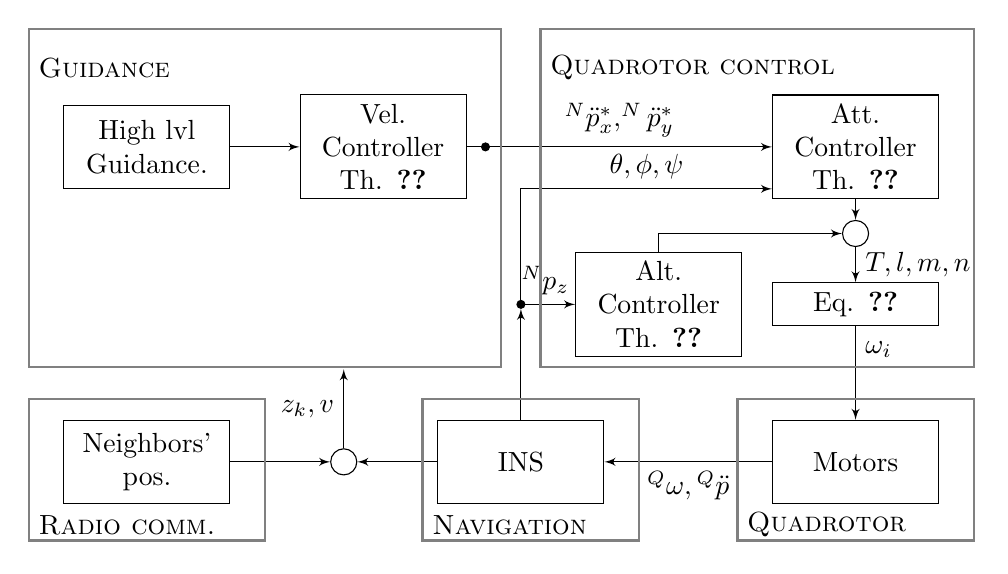
\begin{tikzpicture}[auto, node distance=2cm,>=latex']
	\node [block] (1) {High lvl \\ Guidance.};
	\node [block, draw=white, below of=1] (2) {};
	\node [block, below of=2] (p) {Neighbors' pos.};
	\node [block, right of=1, xshift=1cm] (vel) {Vel. Controller Th. \ref{thm: vel}};
	\node [branch, right of=vel, xshift=-0.7cm] (vb) {};
	\node [block, right of=vel, xshift=4cm] (att) {Att. Controller Th. \ref{thm: att}};
	\node [block, minimum height=1em, below of=att] (w) {Eq. \ref{eq: tlmn2w}};
	\node [block, left of=w, xshift=-0.5cm] (alt) {Alt. Controller Th. \ref{thm: alt}};
	\node [block, below of=w] (mot) {Motors};
	\node [block, left of=mot, xshift=-2.25cm] (nav) {INS};
	\node [sum, below of=att, yshift=0.9cm] (Tlmnb) {};
	\node [sum, left of=nav, xshift=-0.25cm] (navs) {};
	\node [above of=navs, yshift=-0.7cm] (gui) {};
	\node [branch, above of=nav] (navb) {};

	\draw[->] (1) -- (vel);
	\draw[->] (vel) -- node{$^N\ddot p_x^*, ^N\ddot p_y^*$} (att);
	\draw[->] (att) -- (Tlmnb);
	\draw[->] (Tlmnb) -- node{$T,l,m,n$}(w);
	\draw[->] (w) -- node[pos=0.25]{$\omega_i$}(mot);
	\draw[->] (mot) -- node{$^Q\omega, {^Q\ddot p}$}(nav);
	\draw[->] (nav) -- (navb);
	\draw[->] (navb) -- node[pos=0.40]{$^Np_z$}(alt.west);
	\draw[->] (navb) |- node[pos=0.75]{$\theta,\phi,\psi$}($(att.south west)!0.10!(att.north west)$);
%	\draw[->] (2) -| (vb.south);
	\draw[->] (alt.north) |- (Tlmnb.west);
	\draw[->] (nav) -- (navs);
	\draw[->] (p) -- (navs);
	\draw[->] (navs.north) -- node{$z_k, v$} (gui);

	\draw [color=gray,thick](-1.5, -2.8) rectangle (4.5,1.5);
	\node at (-1.5,1) [above=5mm, right=0mm] {\textsc{Guidance}};
	\draw [color=gray,thick](-1.5, -5) rectangle (1.5,-3.2);
	\node at (-1.5,-4.8) [above=5mm, right=0mm] {\textsc{Radio comm.}};
	\draw [color=gray,thick](7.5, -5) rectangle (10.5,-3.2);
	\node at (7.5,-4.8) [above=5mm, right=0mm] {\textsc{Quadrotor}};
	\draw [color=gray,thick](5, -2.8) rectangle (10.5,1.5);
	\node at (5,1) [above=5mm, right=0mm] {\textsc{Quadrotor control}};
	\draw [color=gray,thick](3.5, -5) rectangle (6.25,-3.2);
	\node at (3.5,-4.8) [above=5mm, right=0mm] {\textsc{Navigation}};

\end{tikzpicture}
	\caption{Guidance, Navigation and Control system of the quadrotor. The Guidance block corresponds to the guidance system that generates the desired acceleration signals for the quadrotor in order to accomplish the assigned mission. The quadrotor control block corresponds to the control of the altitude and attitude of the vehicle to track the desired linear accelerations. The Inertial Navigation System (INS) estimates the actual state of the quadrotor which is necessary for the formation and quadrotor controls blocks. The relative positions between neighboring quadrotors could be obtained by communication from the neighbors' INS.}
\label{fig: archCon}
\end{figure}

\section{Assignments}
\label{sec: asi}

\textbf{The algorithms to be designed in the following assigments must be executed locally by each rotorcraft, i.e., there is no a central computer commanding all the vehicles but each one must take its own decissions by running an algorithm with its available information.}
\subsection{Coordinated motion of two rotorcraft with limited sensing}
Consider two rotorcraft $Q_1$ and $Q_2$. The vehicle $Q_1$ knows its position $^Np_1$ but the vehicle $Q_2$ can only measure its altitude $^Np_z$. Both vehicles can measure the distance $||^N(p_1 - p_2)||$ and their relative velocity $^N\dot p_1 - {^N\dot p_2}$. The team must be in formation by having the two vehicles with a relative position $^N(p_1 - p_2) = z$, where $z$ is an (arbitrary offset) vector with zero vertical component, i.e., $z = \begin{bmatrix}z_x & z_y & 0\end{bmatrix}$. Please, design an algorithm such that the center of masses of the team tracks the following ellipse
\begin{equation}
	f(p) = \left(\frac{x-x_o}{a}\right)^2 + \left(\frac{y-y_o}{b}\right)^2 - 1,
\end{equation}
where $\begin{bmatrix}x_o & y_o\end{bmatrix}^T$ is the center of the ellipse and $a,b > 0$ are the length of its axes. The ellipse is located at a fixed altitude $c > 0$. 
	
\begin{itemize}
\item  You can find an (overdetailed) report/reference on the guidance vector field explained in class in \cite{icra17}.
\item $Q_1$ might be a leader executing a path tracking algorithm, and $Q_2$ a follower executing a trajectory tracking algorithm.
\item If you want them to start with a nice initial condition before the \emph{leader-following} stage. You might consider to execute a displacement-based consensus algorithm for controlling the relative position $z$ between $Q_1$ and $Q_2$.
\end{itemize}

\subsection{Tracking and enclosing a target with perfect sensing}
Consider three rotorcraft $Q_1$, $Q_2$ and $Q_3$, and a moving target $Q_t$ at a constant altitude $t_z > 0$ with velocity $\dot p_t = \begin{bmatrix}v_x & v_y & 0\end{bmatrix}$. All our vehicles $Q_1$, $Q_2$ and $Q_3$ know the altitude of the target, and can measure their relative positions w.r.t the target, i.e., $^N(p_{\{1,2,3\}} - p_t)$, and their relative velocities $^N\dot p_{\{1,2,3\}} - {^N\dot p_t}$. Please, design an algorithm such that $Q_1$, $Q_2$ and $Q_3$ describe a circumference around $Q_t$, and $Q_1$, $Q_2$ and $Q_3$ can control their intervehicle angle in the circumference. The angle of $Q_1$ in the circle is just $atan2({^Np}_y,{^Np}_x)$, and the interangle is the subtraction of two angles coming from two vehicles, i.e., we control the relative angle between vehicles in the circle.
	
\begin{itemize}
\item This is a path tracking problem where the center of the circle is moving with a constant velocity.
\item A reference on how to control the position of a team of vehicles on a circle \cite{iros17}. It is just a consensus algorithm on the intervehicle angle of the circumference.
\end{itemize}

\subsection{Formation control for a team of rotorcraft with biased actuators}
Consider three rotorcraft $Q_1, Q_2$ and $Q_3$. Each rotorcraft has a biased velocity command, i.e.,
\begin{equation}
\dot p_i = u_i + b_i,
\end{equation}
where $b_i\in\mathbb{R}$ is an arbitrary \textbf{unknown} bias. All the rotorcraft can measure their absolute positions $^Np_i$, and they have the capability of sharing information, e.g., one rotorcraft can communicate its position to another one. Please, design an algorithm that both, estimate the biases, and exploit displacement-based consensus to achieve an equilateral triangle.
\begin{itemize}
\item You might want to split the task into two stages. The vehicles can estimate first their biases, and once they are \emph{happy}, then start with the consensus algorithm.
\end{itemize}
 
\begin{appendix}
Some advices for the assigment:
\begin{itemize}
	\item The vehicles cannot handle arbitrarily high speeds. Watch out with yor commanded signals.
	\item To speed up simulations you might not want to play the animations but just the final plots from the logs.
	\item Try to understand first the given examples in PyCopter.
	\item Iterate your strategy to implement the algorithms and your final report with the teacher as much as you can.
\end{itemize}
\end{appendix}


\bibliographystyle{IEEEtran}
\bibliography{biblio.bib}

\end{document}
